% !TEX TS-program = pdflatex
% !TEX encoding = UTF-8 Unicode

% This is a simple template for a LaTeX document using the "article" class.
% See "book", "report", "letter" for other types of document.

\documentclass[11pt]{article} % use larger type; default would be 10pt

\usepackage[utf8]{inputenc} % set input encoding (not needed with XeLaTeX)
\usepackage[spanish]{babel}

%%% Examples of Article customizations
% These packages are optional, depending whether you want the features they provide.
% See the LaTeX Companion or other references for full information.

%%% PAGE DIMENSIONS
\usepackage{geometry} % to change the page dimensions
\geometry{a4paper} % or letterpaper (US) or a5paper or....
% \geometry{margin=2in} % for example, change the margins to 2 inches all round
% \geometry{landscape} % set up the page for landscape
%   read geometry.pdf for detailed page layout information

\usepackage{graphicx} % support the \includegraphics command and options
\usepackage[outdir=./]{epstopdf}
% \usepackage[parfill]{parskip} % Activate to begin paragraphs with an empty line rather than an indent

%%% PACKAGES
\usepackage{booktabs} % for much better looking tables
\usepackage{array} % for better arrays (eg matrices) in maths
\usepackage{paralist} % very flexible & customisable lists (eg. enumerate/itemize, etc.)
\usepackage{verbatim} % adds environment for commenting out blocks of text & for better verbatim
%\usepackage{subfig} % make it possible to include more than one captioned figure/table in a single float
\usepackage{subcaption}
\usepackage{url}
\usepackage{diagbox}
\usepackage{amsmath}
\usepackage{pdfpages}
% These packages are all incorporated in the memoir class to one degree or another...

%%% HEADERS & FOOTERS
\usepackage{fancyhdr} % This should be set AFTER setting up the page geometry
\pagestyle{fancy} % options: empty , plain , fancy
\renewcommand{\headrulewidth}{0pt} % customise the layout...
\lhead{}\chead{}\rhead{}
\lfoot{}\cfoot{\thepage}\rfoot{}

%%% SECTION TITLE APPEARANCE
\usepackage{sectsty}
\allsectionsfont{\sffamily\mdseries\upshape} % (See the fntguide.pdf for font help)
% (This matches ConTeXt defaults)

%%% ToC (table of contents) APPEARANCE
\usepackage[nottoc,notlof,notlot]{tocbibind} % Put the bibliography in the ToC
\usepackage[titles,subfigure]{tocloft} % Alter the style of the Table of Contents
\renewcommand{\cftsecfont}{\rmfamily\mdseries\upshape}
\renewcommand{\cftsecpagefont}{\rmfamily\mdseries\upshape} % No bold!

%%% END Article customizations

%%% The "real" document content comes below...

\title{CLP Lab 1 Report}
\author{Albert Aparicio Isarn\\
	\url{albert.aparicio.isarn@alu-etsetb.upc.edu}
	\and 
	Héctor Esteban\\
	\url{hect.esteban@gmail.com}}
\date{} % Activate to display a given date or no date (if empty),
         % otherwise the current date is printed 

\begin{document}
\maketitle

\textbf{Nota:} Al final del documento se encuentra la resolución del estudio previo.

\section[Parte 1 - ROC]{Análisis de curvas ROC}

En las tablas \ref{tab:p1:linear} y \ref{tab:p1:quadratic} se muestran las probabilidades de error para los clasificadores Lineal y Cuadrático, respectivamente.
\begin{table}[h]
	\begin{center}
		\begin{tabular}{| l | c | c | c | c |}
			\hline
			\diagbox[width=8em]{\textbf{Clase}}{\textbf{SNR}} & \textbf{3 dB} & \textbf{0 dB} & \textbf{-3 dB} & {-10 dB} \\
			\hline
			\textbf{Clase 1} & $ 5 \cdot 10^{-3} $ & $ 0.042 $ & $ 0.107$ & 0.3 \\
			\hline
			\textbf{Clase 2} & $ 8 \cdot 10^{-3} $ & $ 0.034 $ & $ 0.106 $ & 0.31 	\\
			\hline
		\end{tabular}
		\caption{Probabilidades de error para el clasificador Lineal (LC)}
		\label{tab:p1:linear}
	\end{center}
\end{table}

\begin{table}[h]
	\begin{center}
		\begin{tabular}{| l | c | c | c | c |}
			\hline
			\diagbox[width=8em]{\textbf{Clase}}{\textbf{SNR}} & \textbf{3 dB} & \textbf{0 dB} & \textbf{-3 dB} & {-10 dB} \\
			\hline
			\textbf{Clase 1} & $ 7 \cdot 10^{-3} $ & $ 0.041 $ & $ 0.114$ & 0.292 \\
			\hline
			\textbf{Clase 2} & $ 3 \cdot 10^{-3} $ & $ 0.036 $ & $ 0.118 $ & 0.306 	\\
			\hline
		\end{tabular}
		\caption{Probabilidades de error para el clasificador Cuadrático (QC)}
		\label{tab:p1:quadratic}
	\end{center}
\end{table}

En las figuras \ref{fig:p1:roc:-3} y \ref{fig:p1:roc:-10} se muestran las curvas ROC para los casos de -3 y -10 dB, respectivamente.

\begin{figure}[h]
	\centering
	\begin{subfigure}[b]{\textwidth}
		\centering
		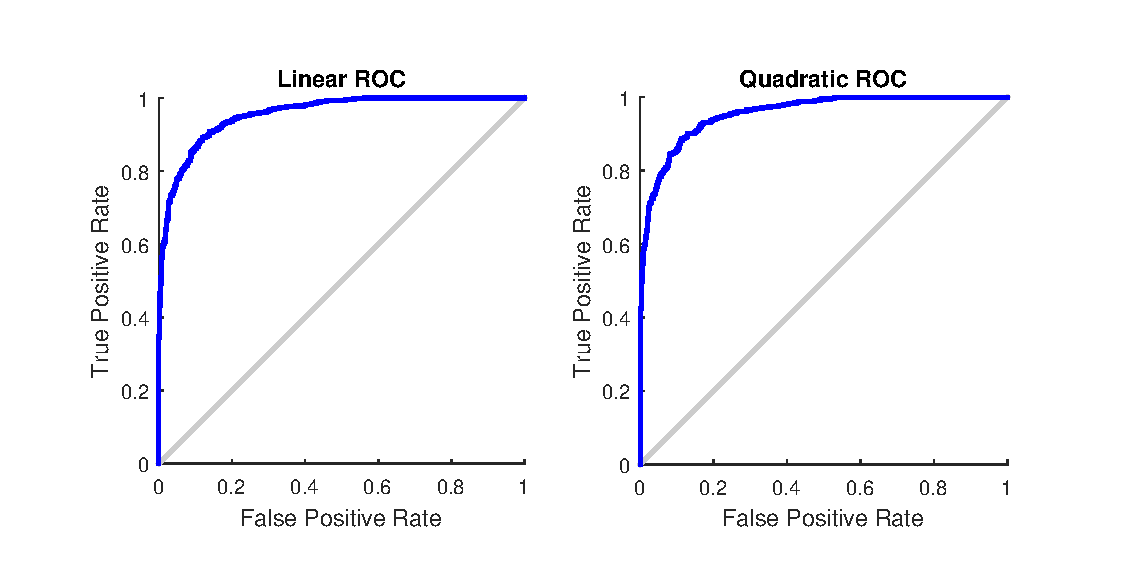
\includegraphics[width=\textwidth]{../Part_1/ROC_-3.eps}
		\caption[]{\small SNR $ = -3 dB$}
		\label{fig:p1:roc:-3}
	\end{subfigure}
	
	\begin{subfigure}[b]{\textwidth}
		\centering
		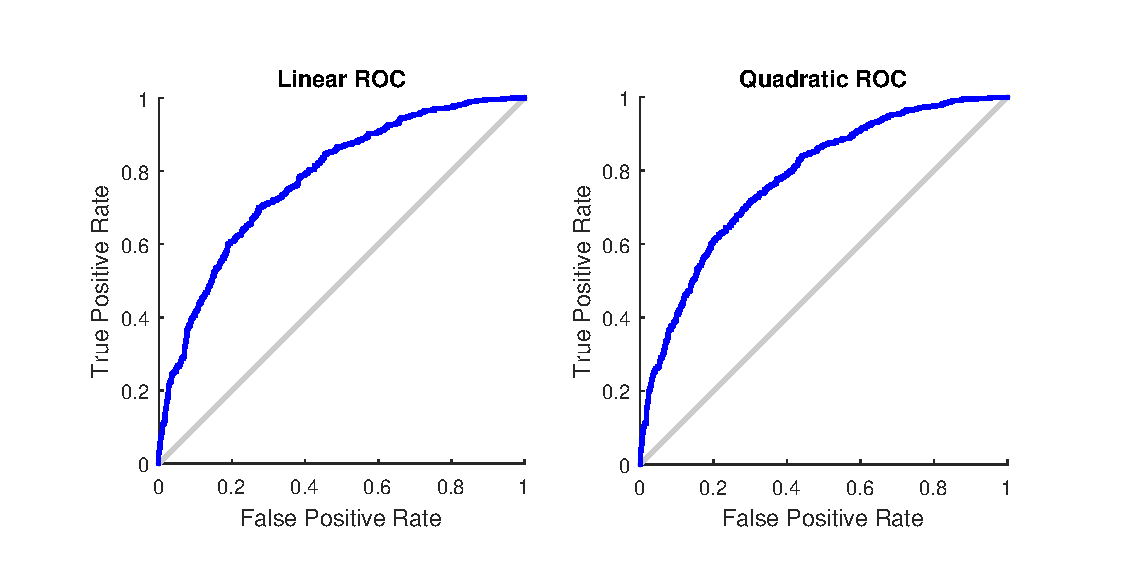
\includegraphics[width=\textwidth]{../Part_1/ROC_-10.eps}
		\caption[]{\small SNR $ = -10 dB$} 
		\label{fig:p1:roc:-10}
	\end{subfigure}
	\label{fig:p1}
	\caption{Curvas ROC de los clasificadores Lineal y Cuadrático}
\end{figure}

Las variaciones en las distancias de Mahalanobis son debidas al error en las estimaciones de las medias y covarianzas de los vectores de las clases hechas por la función 'mahal'.

\clearpage

\section[Parte 2 - Autovalores]{Autovalores de matriz de covarianza y
	forma de los clusters}

\subsection[Caso 2]{QPSK Caso 2}

En las figuras \ref{fig:c2:ro00} y \ref{fig:c2:ro05} se muestran los diagramas de scatter y sus fronteras de decisión, para los casos $\rho = 0$ y $\rho = +0.5$, respectivamente.

\begin{figure}%[h]
	\centering
	\begin{subfigure}[b]{0.475\textwidth}
		\centering
		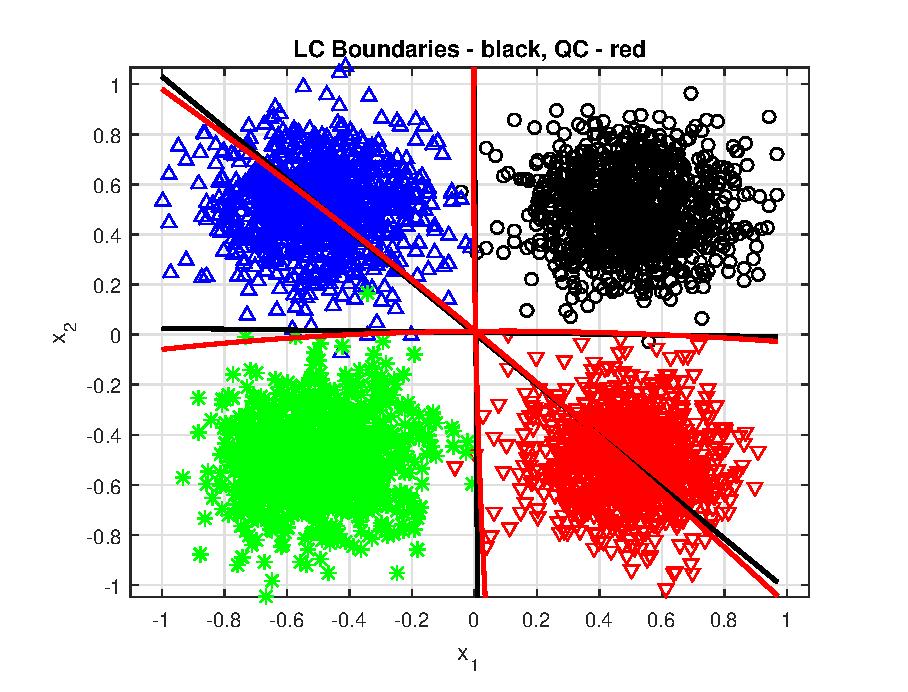
\includegraphics[width=\textwidth]{../Part_2/ro00_scatter.eps}
		\caption[]{\small $\rho = 0$}
		\label{fig:c2:ro00}
	\end{subfigure}
	\quad
	\begin{subfigure}[b]{0.475\textwidth}
		\centering
		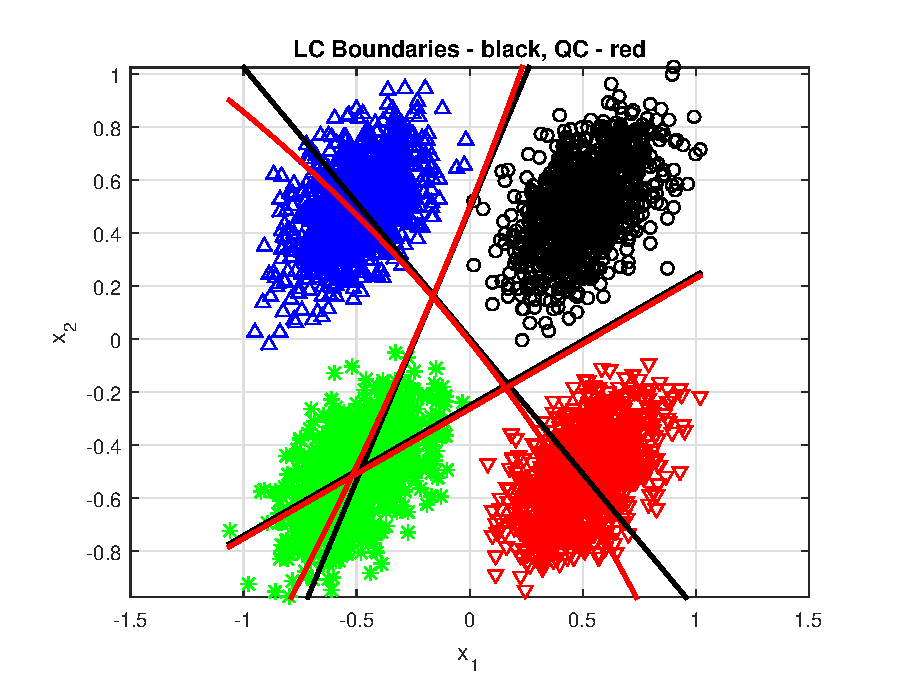
\includegraphics[width=\textwidth]{../Part_2/ro05_scatter.eps}
		\caption[]{\small $\rho = 0.5$} 
		\label{fig:c2:ro05}
	\end{subfigure}
	\label{fig:c2:scatter}
	\caption{Diagramas \emph{Scatter} y sus fronteras de decisión para el caso 2.}
\end{figure}

La matriz de confusión para el clasificador lineal en el caso $\rho = 0$ se muestra en \eqref{eq:c2:linear:00}:

\begin{equation} \label{eq:c2:linear:00}
\left( \begin{array}{cccc}
999 & 1 & 0 & 0 \\
1 & 999 & 0 & 0 \\
0 & 0 & 999 & 1 \\
0 & 0 & 2 & 998 \\ 
\end{array} \right)
\end{equation}

En \eqref{eq:c2:quad:00} se muestra la matriz del clasificador cuadrático:

\begin{equation} \label{eq:c2:quad:00}
\left( \begin{array}{cccc}
998 & 2 & 0 & 0 \\
0 & 1000 & 0 &0 \\
0 & 0 & 999 & 1 \\
0 & 0 & 2 & 998 \\ 
\end{array} \right)
\end{equation}

Las matrices de confusión para los clasificadores lineal y cuadrático, en el caso $\rho = 0.5$ se muestran en \eqref{eq:c2:linear:05} y \eqref{eq:c2:quad:05}, respectivamente:

\begin{equation} \label{eq:c2:linear:05}
\left( \begin{array}{cccc}
999 & 0 & 0 & 1 \\
0 & 1000 & 0 & 0 \\
0 & 0 & 1000 & 0 \\
0 & 0 & 0 & 1000 \\ 
\end{array} \right)
\end{equation}

\begin{equation} \label{eq:c2:quad:05}
\left( \begin{array}{cccc}
999 & 0 & 0 & 1 \\
0 & 1000 & 0 & 0 \\
0 & 0 & 1000 & 0 \\
0 & 0 & 0 & 1000 \\ 
\end{array} \right)
\end{equation}

Las probabilidades de error para los casos $\rho = 0$ y $\rho = 0.5$ están organizadas en las Tablas \ref{tab:c2:00} y \ref{tab:c2:05}, respectivamente:

\begin{table}[h]
	\begin{center}
		\begin{tabular}{| l | c | c | c | c |}
			\hline
			\diagbox[width=11em]{\textbf{Clasificador}}{\textbf{Clase}} & \textbf{1} & \textbf{2} & \textbf{3} & {4} \\
			\hline
			\textbf{Lineal (LC)} & $ 1 \cdot 10^{-3} $ & $ 1 \cdot 10^{-3} $ & $ 1 \cdot 10^{-3} $ & $ 2 \cdot 10^{-3} $ \\
			\hline
			\textbf{Cuadrático (QC)} & $ 2 \cdot 10^{-3} $ & $ 0 $ & $ 1 \cdot 10^{-3} $ & $ 2 \cdot 10^{-3} $ 	\\
			\hline
		\end{tabular}
		\caption{Probabilidades de error para el caso $\rho = 0$}
		\label{tab:c2:00}
	\end{center}
\end{table}

\begin{table}[h]
	\begin{center}
		\begin{tabular}{| l | c | c | c | c |}
			\hline
			\diagbox[width=11em]{\textbf{Clasificador}}{\textbf{Clase}} & \textbf{1} & \textbf{2} & \textbf{3} & {4} \\
			\hline
			\textbf{Lineal (LC)} & $ 1 \cdot 10^{-3} $ & $ 0 $ & $ 0 $ & $ 0 $ \\
			\hline
			\textbf{Cuadrático (QC)} & $ 1 \cdot 10^{-3} $ & $ 0 $ & $ 0 $ & $ 0 $ \\
			\hline
		\end{tabular}
		\caption{Probabilidades de error para el caso $\rho = 0.5$}
		\label{tab:c2:05}
	\end{center}
\end{table}

Observando las matrices de confusión se puede apreciar como los resultados para $\rho = 0$ y $\rho = 0.5$ son prácticamente iguales. Cabe destacar que se produce una diferencia en las formas de las Gausianas y de las fronteras en ambos casos debido a que en el caso de $\rho = 0$ los dos autovalores de la matriz coinciden con lo que provocan una gausiana totalmente circular, en cambio para $\rho = 0.5$ su forma es parecida a la de una elipse.

%\newpage

\subsection[Caso 3]{QPSK Caso 3}

Las probabilidades de error al aplicar LC y QC, para los dos valores de SNR se muestran en las Tablas \ref{tab:c3:snr10} y \ref{tab:c3:snr5}:

\begin{table}[h]
	\begin{center}
		\begin{tabular}{| l | c | c | c | c |}
			\hline
			\diagbox[width=11em]{\textbf{Clasificador}}{\textbf{Clase}} & \textbf{1} & \textbf{2} & \textbf{3} & {4} \\
			\hline
			\textbf{Lineal (LC)} & $ 0 $ & $ 6 \cdot 10^{-3} $ & $ 5 \cdot 10^{-3} $ & $ 0 $ \\
			\hline
			\textbf{Cuadrático (QC)} & $ 0 $ & $ 3 \cdot 10^{-3} $ & $ 0 $ & $ 0 $ 	\\
			\hline
		\end{tabular}
		\caption{Probabilidades de error para $SNR = 10 dB$}
		\label{tab:c3:snr10}
	\end{center}
\end{table}

\begin{table}[h]
	\begin{center}
		\begin{tabular}{| l | c | c | c | c |}
			\hline
			\diagbox[width=11em]{\textbf{Clasificador}}{\textbf{Clase}} & \textbf{1} & \textbf{2} & \textbf{3} & {4} \\
			\hline
			\textbf{Lineal (LC)} & $ 0.064 $ & $ 0.094 $ & $ 0.087 $ & $ 0.037 $ \\
			\hline
			\textbf{Cuadrático (QC)} & $ 0.073 $ & $ 0.064 $ & $ 0.067 $ & $ 0.044 $ \\
			
			\hline
		\end{tabular}
		\caption{Probabilidades de error para $SNR = 5 dB$}
		\label{tab:c3:snr5}
	\end{center}
\end{table}

Los autovalores teóricos y prácticos están dispuestos en las Tablas \ref{tab:c3:eig:teor} y \ref{tab:c3:eig:prac}. Para obtener los valores teóricos, la varianza se ha obtenido de las diagonales de la matriz de covarianza:

\begin{table}[h]
	\begin{center}
		\begin{tabular}{| c | c | c | c | c |}
			\hline
			\diagbox[width=11em]{\textbf{Autovalor}}{\textbf{Clase}} & \textbf{1} & \textbf{2} & \textbf{3} & {4} \\
			\hline
			\multicolumn{5}{| c |}{SNR $= 10dB$}\\
            \hline
            $\lambda_1$ & $0.0375$ & $0.0250$ & $0.0125$ & $0.0450$ \\
            \hline
            $\lambda_2$ & $0.0125$ & $0.0250$ & $0.0375$ & $0.0050$ \\
 			\hline
 			\multicolumn{5}{| c |}{SNR $= 5dB$}\\
            \hline
            $\lambda_1$ & $0.1187$ & $0.0791$ & $0.0396$ & $0.1424$ \\
            \hline
            $\lambda_2$ & $0.0396$ & $0.0791$ & $0.1187$ & $0.0158$ \\
            \hline
		\end{tabular}
		\caption{Autovalores teóricos para los dos valores de SNR}
		\label{tab:c3:eig:teor}
	\end{center}
\end{table}

\begin{table}[h]
	\begin{center}
		\begin{tabular}{| c | c | c | c | c |}
			\hline
			\diagbox[width=11em]{\textbf{Autovalor}}{\textbf{Clase}} & \textbf{1} & \textbf{2} & \textbf{3} & {4} \\
			\hline
			\multicolumn{5}{| c |}{SNR $= 10dB$}\\
			\hline
            $\lambda_1$ & $0.0375$ & $0.0250$ & $0.0375$ & $0.0450$ \\
			\hline
            $\lambda_2$ & $0.0125$ & $0.0250$ & $0.0125$ & $0.0050$ \\
			\hline
			\multicolumn{5}{| c |}{SNR $= 5dB$}\\
			\hline
            $\lambda_1$ & $0.1187$ & $0.0791$ & $0.0396$ & $0.1424$ \\
			\hline
            $\lambda_2$ & $0.0396$ & $0.0791$ & $0.1187$ & $0.0158$ \\
 			\hline
		\end{tabular}
		\caption{Autovalores prácticos para los dos valores de SNR}
		\label{tab:c3:eig:prac}
	\end{center}
\end{table}

En las figuras \ref{fig:c3:snr05} y \ref{fig:c3:snr10}  se pueden ver los diagramas Scatter para los dos valores de SNR trabajados:

\begin{figure}[h]
	\centering
	\begin{subfigure}[b]{0.475 \textwidth}
		\centering
		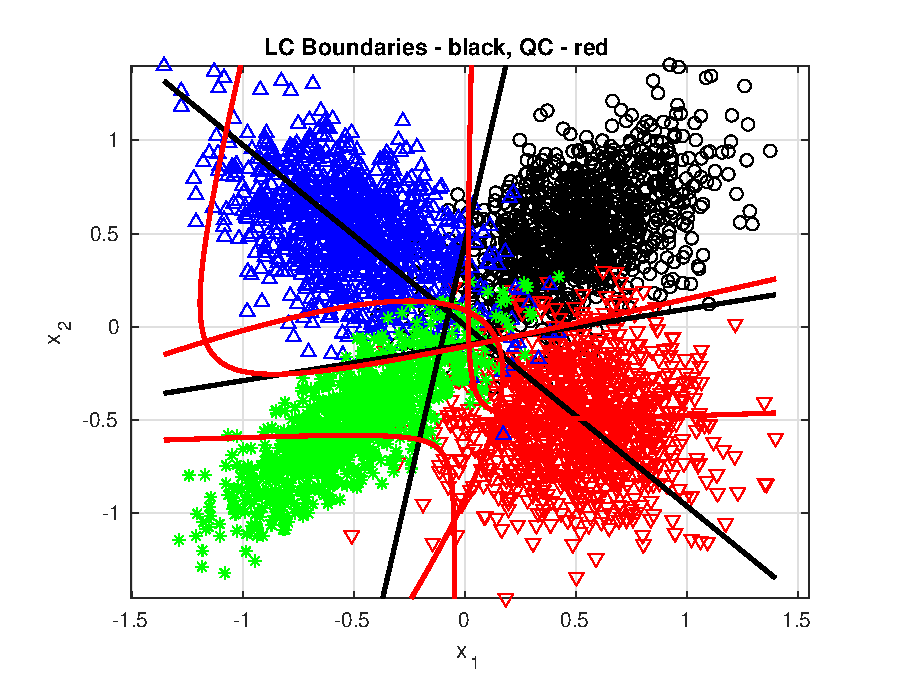
\includegraphics[width=\textwidth]{../Part_2/caso3_05dB.eps}
		\caption[]{\small SNR $= 5dB$}
		\label{fig:c3:snr05}
	\end{subfigure}
	\quad
	\begin{subfigure}[b]{0.475 \textwidth}
		\centering
		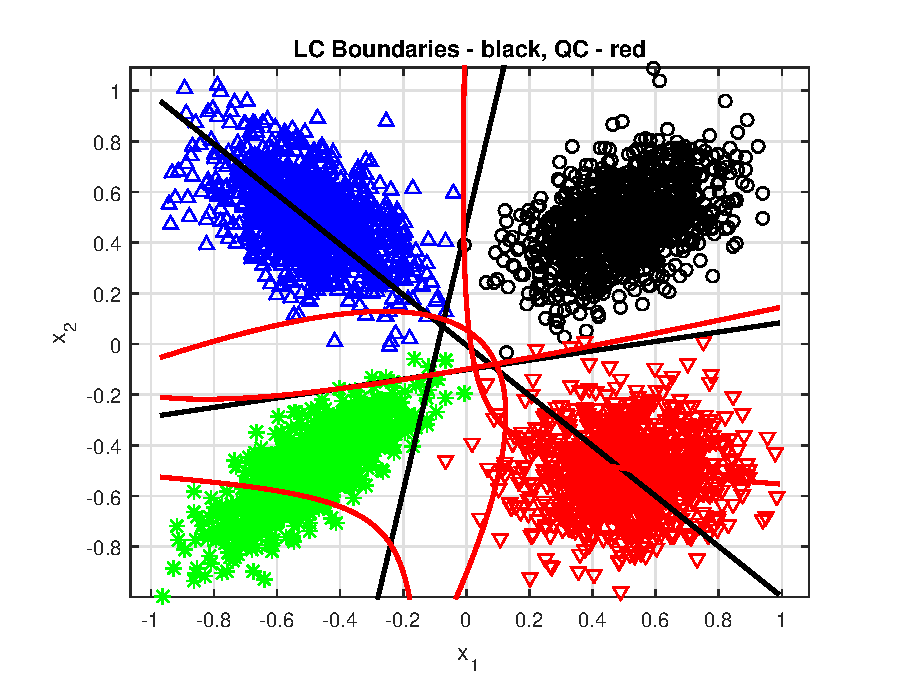
\includegraphics[width=\textwidth]{../Part_2/caso3_10dB.eps}
		\caption[]{\small SNR $= 10dB$} 
		\label{fig:c3:snr10}
	\end{subfigure}
	\caption{Diagramas \emph{Scatter} y sus fronteras de decisión para los dos valores de SNR del caso 3.}
	\label{fig:c3:scatter}
\end{figure}

\newpage
\subsubsection{Multiplicar covarianza de la 1ra clase}

Al aumentar el valor de $\sigma$ de la clase 1 hemos aumentado su rango de afluencia por todo el plano, con lo que resulta imposible separarla de las demás clases por lineas rectas. En cambio, si utilizamos clasificadores cuadráticos estos nos permiten envolver de una manera determinada las clases y así conseguir la separación deseada. En nuestro ejemplo obtuvimos un error provocado por el clasificador lineal de $0.2075$ y de $0.005$ para el clasificador cuadrático. También se aprecia que debido a los valores no nulos de $\rho$ en los símbolos 1,3 y 4, sus formas no son totalmente circulares.

El resultado se muestra en la figura \ref{fig:c3:mult}:

\begin{figure}[h]
	\centering
	\begin{subfigure}[b]{0.475 \textwidth}
		\centering
		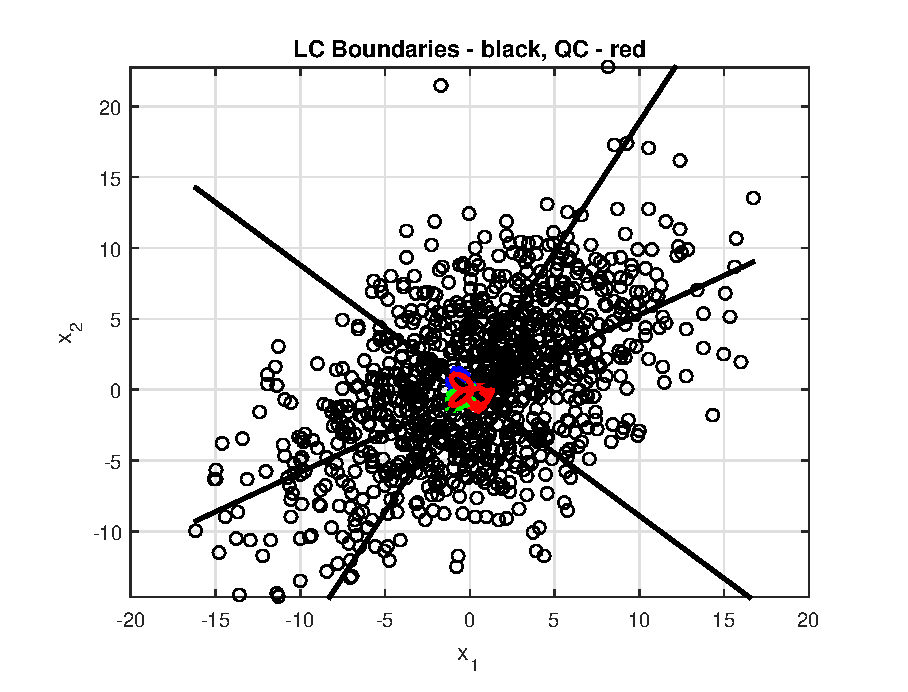
\includegraphics[width=\textwidth]{../Part_2/caso3_sigma30_nozoom.eps}
		\caption[]{\small Diagrama \emph{Scatter} con las fronteras de decisión a tamaño original}
		\label{fig:c3:mult:nozoom}
	\end{subfigure}
	\quad
	\begin{subfigure}[b]{0.475 \textwidth}
		\centering
		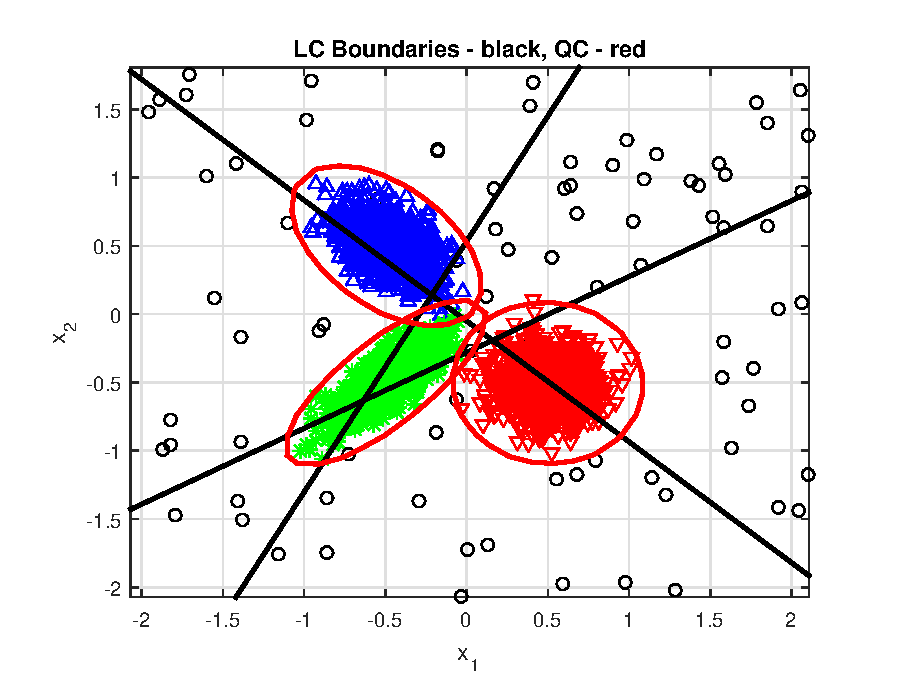
\includegraphics[width=\textwidth]{../Part_2/caso3_sigma30_zoom.eps}
		\caption[]{\small Diagrama \emph{Scatter} con la zona central ampliada, mostrando las fonteras cuadráticas elípticas} 
		\label{fig:c3:mult:zoom}
	\end{subfigure}
	\caption{Diagramas \emph{Scatter} con la covarianza de la 1ra clase ampliada}
	\label{fig:c3:mult}
\end{figure}

\clearpage

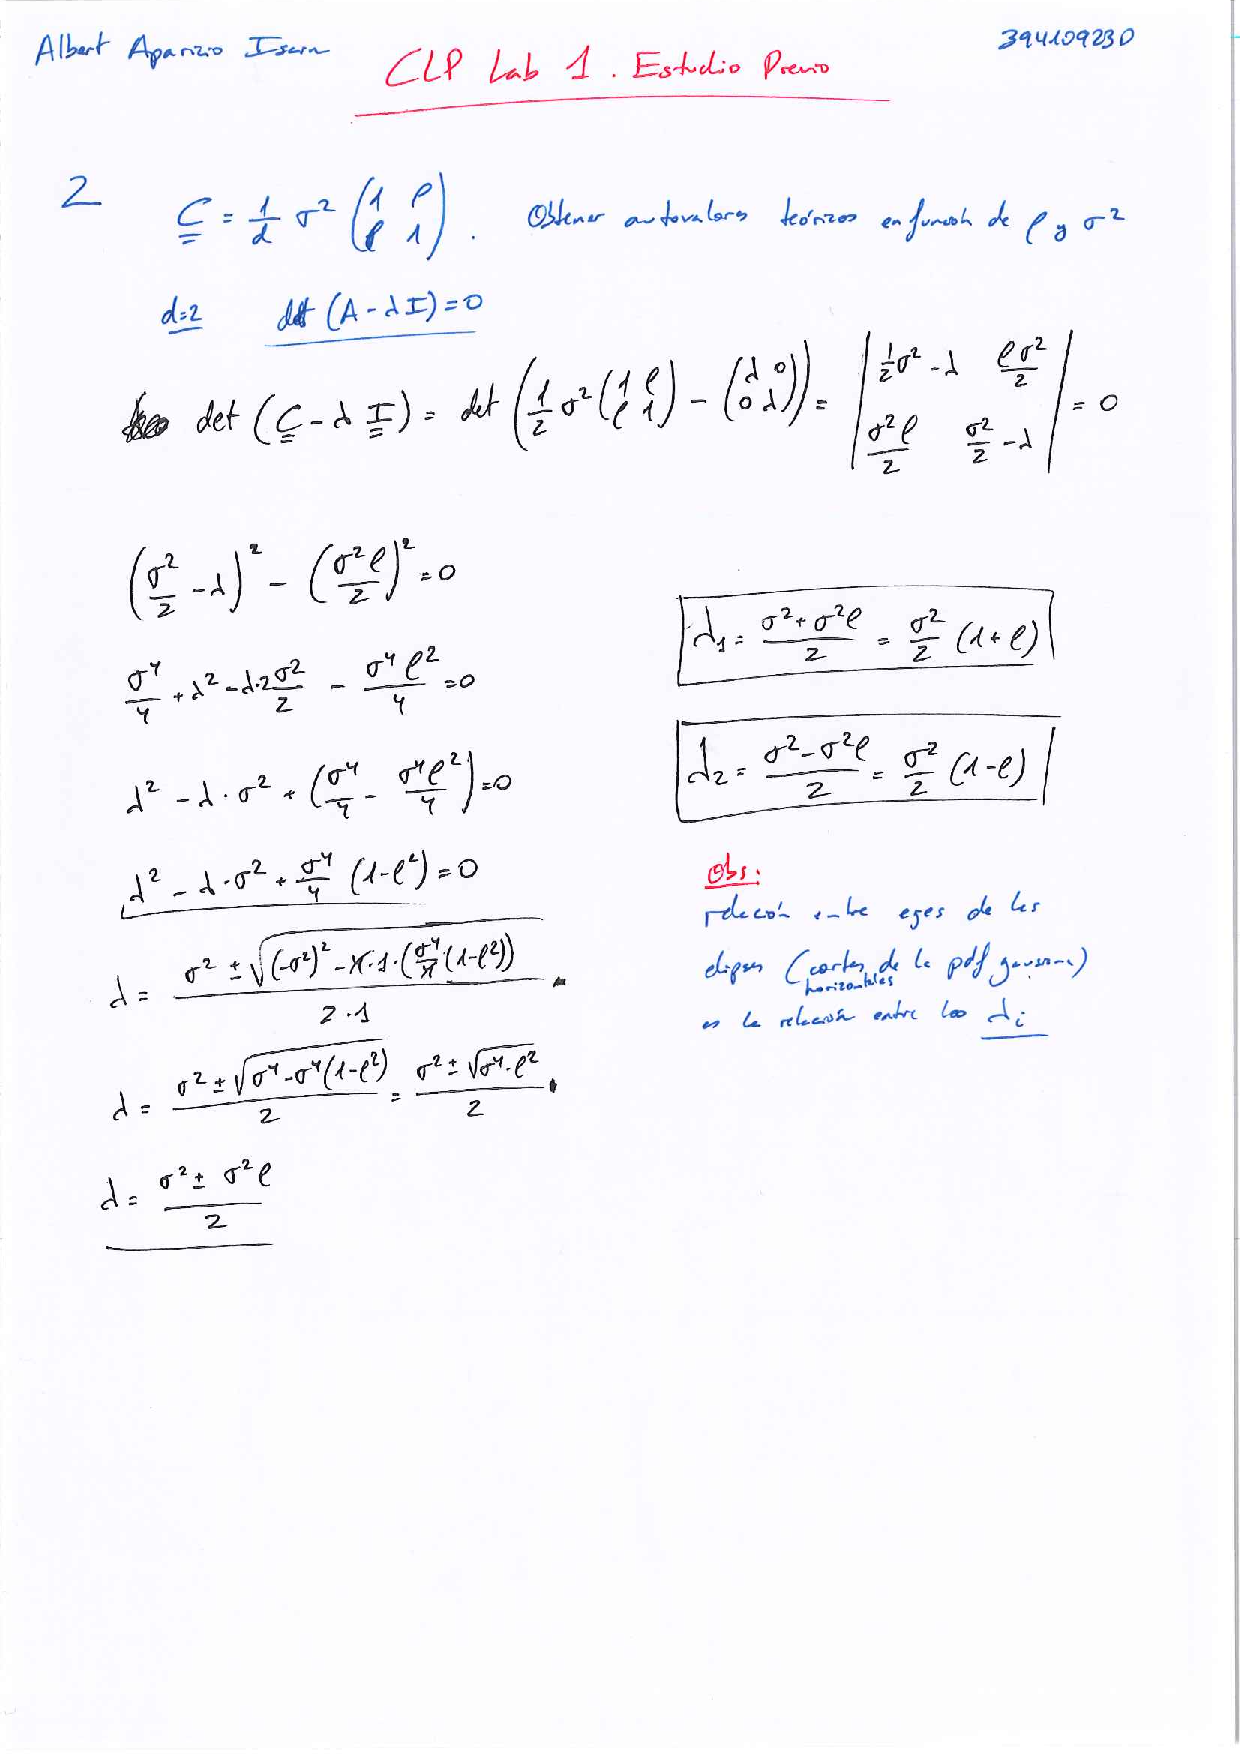
\includepdf[pages={1}]{../CLP_Prac1_Estudio-Previo.pdf}

\end{document}
